\documentclass[a4,center,fleqn]{NAR}

% Enter dates of publication
\copyrightyear{2008}
\pubdate{31 July 2009}
\pubyear{2013}
\jvolume{37}
\jissue{12}

%\articlesubtype{This is the article type (optional)}

\begin{document}

\title{TagDust2 - a program to extract and correctly label next generation sequencing reads.}

\author{%
Timo Lassmann\,$^{1}$%
\footnote{To whom correspondence should be addressed.
Tel: +44 000 0000000; Fax: +44 000 0000000; Email: xxx@yyyy.ac.zz}}

\address{%
$^{1}$Division of Genomic Technologies, Center for Life Science Technologies,
RIKEN Yokohama Institute
1-7-22 Suehiro-cho, Tsurumi-ku, Yokohama
230-0045 Kanagawa, Japan 
}
% Affiliation must include:
% Department name, institution name, full road and district address,
% state, Zip or postal code, country

\history{%
Received January 1, 2013;
Revised February 1, 2013;
Accepted March 1, 2013}

\maketitle

\begin{abstract}

Arguably the most basic step basic step in the processing of next generation sequence (NGS) involves extracting mappable reads from raw reads produced by the sequencer. The presence of barcodes, fingerprints and artifacts such as adapter dimers makes this step non-trivial. 

TagDust allows users to specify the expected architecture of a read and converts it into a hidden Markov model. The latter can assign sequences to a particular barcode (or index) even in the presence of sequencing errors. Artifactual sequences, which by definition do not not match the architecture are automatically discarded.

\end{abstract}


\section{Introduction}

Next generation sequencing has greatly accelerated the accumulation of genomics data. Different protocols targeting the genome, dpi-genome and transcriptions are commonly used. In essence all protocols capture biological sequences of interest, add sequences to make the library subject able to NGS sequencing. The great increase in sequencing depth allows for the sequencing of multiple samples one channel. In this case additional sequences or barcodes are added to the reads allowing for the identification of the original samples after sequencing. A key research area where such multiplexing is essential is single cell sequencing. In addition to this recent protocols have added random sequences of a specific length to the reads allowing to identify PCR duplicates [STEN]. 


Increasing the length of the accessory sequences also increases the chances of sequencing errors occurring within them. In the best case this leads to some sequences being lost to the downstream analysis, but in the worse case sequences can be mixed up between experiments leading to analytical noise. 

Recently, I introduced TagDust to remove artifactual sequences.

Luckily this problem is very similar to many problems in biological sequence analysis. Here I address this problem by using hidden Markov models. The program TagDust2 allows users to specify the expected order of stuff in the reads. As a by product all sequences not matching the expected sequence of read segments can be easily identified and discarded. 
% **************************************************************
% Keep this command to avoid text of first page running into the
% first page footnotes
\enlargethispage{-65.1pt}
% **************************************************************

Text. Text. Text. Text. Text. Text.
Text. Text. Text. Text. Text. Text. Text. Text. Text. Text. Text.
Text. Text. Text. Text. Text. Text. Text. Text. Text. Text. Text.
Text. Text. Text. Text. Text. Text. Text. Text. Text. Text. Text.
Text. Text. Text. Text. Text. Text. Text. Text. Text. Text. Text.
Text. Text. Text. Text. Text. Text. Text. Text. Text. Text. Text.
Text. Text. Text. Text. Text. Text. Text. Text. Text. Text. Text.
Text. Text. Text. Text. Text. Text. Text. Text. Text. Text. Text.
Text. Text. Text. Text. Text. Text. Text. Text. Text. Text. Text.
Text. Text. Text. Text. Text. Text. Text. Text. Text. Text. Text.
Text. Text. Text. Text. Text. Text. Text. Text. Text. Text. Text.
Text. Text. Text. Text. Text. Text. Text. Text. Text. Text. Text.
Text. Text. Text. Text. Text. Text. Text. Text. Text. Text. Text.
Text. Text. Text. Text. Text. Text. Text. Text. Text. Text. Text.
Text. Text. Text. Text. Text. Text. Text. Text. Text. Text. Text.
Text. Text. Text. Text. Text. Text. Text. Text. Text. Text. Text.
Text. Text. Text. Text.
Text \cite{2,3}.

Text. Text. Text. Text. Text. Text. Text. Text. Text. Text. Text.
Text. Text. Text. Text. Text. Text. Text. Text. Text. Text. Text.
Text. Text. Text. Text. Text. Text. Text. Text. Text. Text. Text.
Text. Text. Text. Text. Text. Text. Text. Text. Text. Text. Text.
Text. Text. Text. Text. Text. Text. Text. Text. Text. Text. Text.
Text. Text. Text. Text. Text. Text. Text. Text. Text. Text. Text.
Text. Text. Text. Text. Text. Text. Text. Text. Text. Text. Text.
Text. Text. Text. Text. Text. Text. Text. Text. Text. Text. Text.
Text. Text. Text. Text. Text. Text. Text. Text. Text. Text. Text.
Text. Text. Text. Text. Text. Text. Text. Text. Text. Text.
Text. Text. Text. Text. Text. Text. Text. Text. Text. Text. Text.
Text. Text. Text. Text. Text. Text. Text. Text. Text. Text. Text.
Text. Text. Text. Text. Text. Text. Text. Text. Text. Text. Text.
Text. Text. Text. Text. Text. Text. Text. Text. Text. Text. Text.
Text. Text. Text. Text. Text. Text. Text. Text. Text. Text. Text.
Text. Text. Text. Text. Text. Text. Text. Text. Text. Text. Text.
Text. Text. Text. Text. Text. Text. Text. Text. Text. Text. Text.
Text. Text. Text. Text. Text. Text. Text. Text. Text. Text. Text.
Text. Text. Text. Text. Text. Text. Text. Text. Text. Text. Text.
Text. Text. Text. Text. Text. Text. Text. Text. Text. Text. Text.
Text. Text. Text. Text. Text. Text. Text. Text. Text. Text. Text.
Text. Text. Text. Text. Text. Text. Text. Text. Text. Text. Text.
Text. Text. Text. Text. Text. Text. Text. Text. Text. Text. Text.
Text. Text. Text. Text. Text. Text. Text. Text.
Text \cite{4}.

\section{MATERIALS AND METHODS}

\subsection{General Approach}

\begin{figure}[t]
\begin{center}
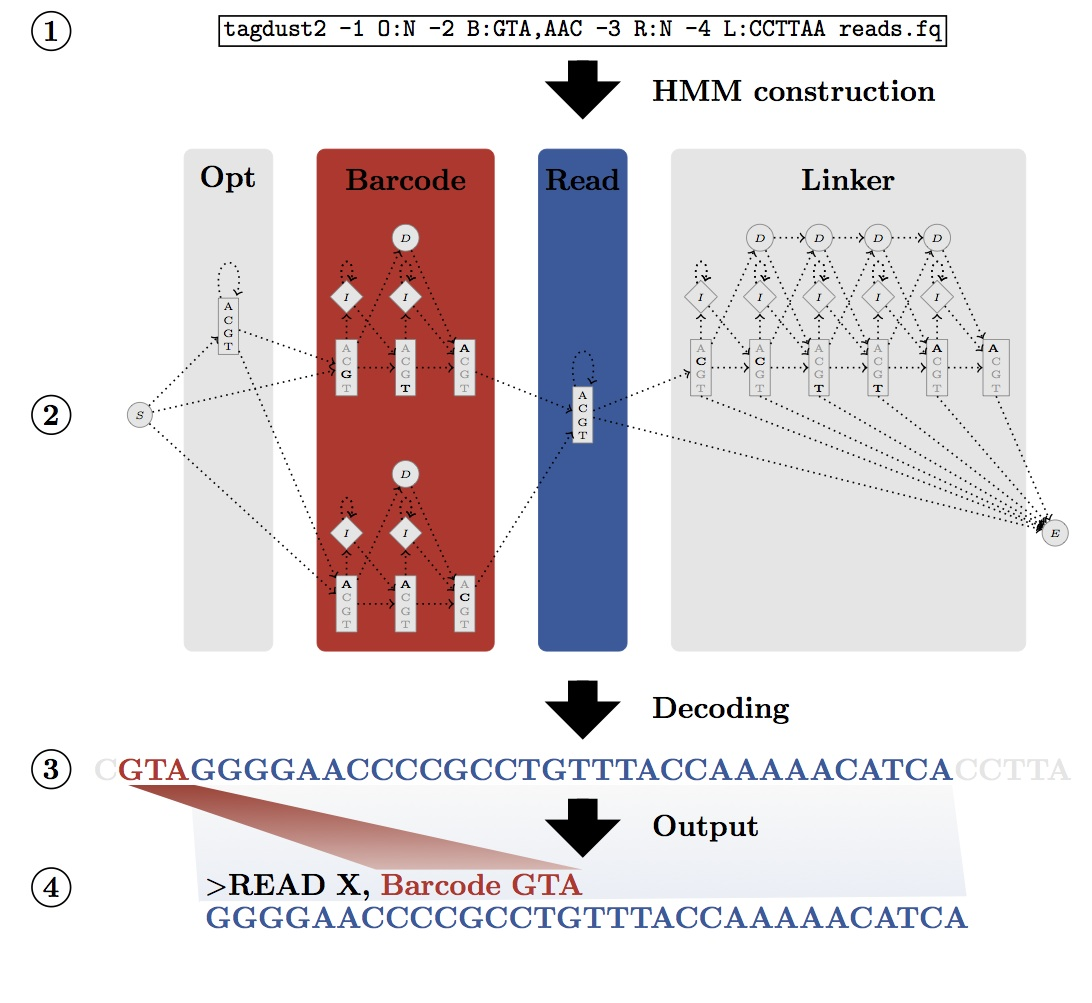
\includegraphics[scale = 0.5]{../figures/figure1.pdf}
\end{center}
\caption{Overview of the TagDust workflow. Sequences are labelled according to the HMM architecture and relevant information written to the output. 
}
\label{figure1}
\end{figure}

TagDust implements a small library of HMMs which we will refer to as segments. Each segment contains a silent start and end state which are used to connect multiple segments. Segments are hand-designed to capture commonly occurring features in raw sequences such as barcode combinations, variable length sequences and so on. For a complete list see table 1. Users can use a simple command line interface to specify the expected sequence of segments in their reads. TagDust automatically constructs a global HMMs from the segments and starts scoring the individual reads (see Figure \ref{figure1}). 

Parameterization... 

Text. Text. Text. Text. Text. Text. Text. Text. Text. Text. Text.
Text. Text. Text. Text. Text. Text. Text. Text. Text. Text. Text.
Text. Text. Text. Text. Text. Text. Text. Text. Text. Text. Text.
Text. Text. Text. Text. Text. Text. Text. Text. Text. Text. Text.
Text. Text. Text. Text. Text. Text. Text. Text. Text. Text. Text.
Text. Text. Text. Text. Text. Text. Text. Text. Text. Text. Text.
Text. Text. Text. Text. Text. Text. Text. Text. Text. Text. Text.
Text. Text. Text. Text. Text. Text. Text. Text. Text. Text. Text.
Text. Text. Text. Text. Text. Text. Text. Text. Text. Text. Text.
Text. Text. Text. Text. Text. Text. Text. Text. Text. Text. Text.
Text. Text. Text. Text. Text. Text. Text. Text. Text. Text. Text.
Text. Text. Text. Text. Text. Text. Text. Text. Text. Text. Text.
Text. Text. Text. Text. Text. Text. Text. Text. Text. Text. Text.
Text. Text. Text. Text. Text. Text. Text. Text. Text. Text. Text.
Text. Text. Text. Text. Text. Text. Text. Text. Text. Text. Text.
Text. Text. Text. Text. Text. Text. Text. Text. Text. Text. Text.
Text. Text. Text. Text. Text. Text. Text. Text. Text. Text. Text.
Text. Text. Text. Text. Text. Text. Text. Text. Text. Text. Text.
Text. Text. Text. Text. Text. Text. Text. Text. Text. Text. Text.
Text. Text. Text. Text. Text. Text. Text. Text. Text. Text. Text.
Text. Text. Text. Text. Text. Text. Text. Text. Text. Text. Text.
Text. Text. Text. Text. Text. Text. Text. Text. Text. Text. Text.
Text. Text. Text. Text. Text. Text. Text. Text. Text. Text. Text.
Text. Text. Text. Text. Text. Text. Text. Text. Text. Text.


\subsubsection{Materials subsubsection one.}

Text. Text. Text. Text. Text. Text. Text. Text. Text. Text. Text.
Text. Text. Text. Text. Text. Text. Text. Text. Text. Text. Text.
Text. Text. Text. Text:
\begin{align}
\mathrm{LD}^r = \frac{\mathrm{LD}}{A_\mathrm{iso}}
= 1.5 S \left( 3 \cos^2 \alpha_i - 1 \right)
\end{align}
Text. Text. Text. Text. Text. Text. Text. Text. Text. Text. Text.
Text. Text. Text. Text. Text. Text. Text. Text. Text. Text. Text.
Text. Text. Text. Text. Text. Text. Text. Text. Text. Text. Text.
Text. Text. Text. Text. Text. Text. Text. Text. Text. Text. Text.
Text. Text. Text. Text. Text. Text. Text. Text. Text. Text. Text.
Text. Text. Text. Text. Text. Text. Text. Text. Text. Text. Text.
Text. Text. Text. Text. Text. Text. Text. Text. Text. Text. Text.
Text. Text. Text. Text. Text. Text. Text. Text. Text. Text. Text.
Text. Text. Text. Text. Text. Text. Text. Text. Text. Text. Text.
Text. Text. Text. Text. Text. Text. Text. Text. Text. Text. Text.
Text. Text. Text. Text. Text. Text. Text. Text. Text. Text. Text.
Text. Text. Text. Text. Text. Text. Text. Text. Text. Text. Text.



\subsection{Sequence scoring} 

TagDust implements the basic forward and backward algorithm as described in \citep{durbin}. For each sequence the logs odds score is defined by the summed probability of all paths (forward score) divided by the probability of a background zero order Markov model. The latter is parameterized based on the length and nucleotide distribution in the input reads. 

\begin{equation}
	S  = log \left(  \frac{P(M)}{P(R)} \right) + log \left(\frac{\sum\limits_{\pi} P(x,\pi | M )}{P(x | R ) } \right)
\end{equation}

The prior probabilities $P(M)$ and  $P(R)$ are set to 0.9 and 0.1 respectively. Finally, the log odds score is converted into a probability using the logistic function:

\begin{equation}
	P(M | x) = \frac{e^S}{1-e^S}
\end{equation}

If barcodes are present TagDust calculated an additional confidence score. At every building block containing multiple transitions from the silent state to HMMs, TagDust calculates the maximum probability of selecting one particular transition:       


\begin{equation}
	V = \max_j \left( \frac{f_s(i)  ( a_{s,m_j} e_{m_j}(x+1) b_{m_j}(i+1)+  a_{s,I_j} e_{I_j}(x+1) b_{I_j}(i+1))}{\sum\limits_{\pi} P(x,\pi | M )}\right)
\end{equation}

where $m_j$ and $I$ are the first match and insert states of a barcode HMM model. In essence this probability reflects how confident we are in selecting one barcode over any other. 

As a default TagDust only extracts reads if $V$ is greater than 0.5 and $P(M | x)$ is greater than 0.99. 

\subsection{Optimal accuracy decoding} 

To obtain the most probably labeling of the sequence, we employ the optimal accuracy decoding algorithm as described in \citep{Kall:2005vg}. To apply this algorithm to our problem define the label probability of a nucleotide by the summed posterior label probabilities of states belonging to a particular HMM building block. A secondary dynamic programming algorithm is used to determine the path with the maximal label probability, constrained by the global HMM architecture. The label probabilities are essentially used as a substitution matrix while the architecture is enforced by the equivalent of gap penalties. 

If fingerprints are present TagDust checks at this stage if the length after decoding matches the users input. If not the read is discarded. 


\subsection{Implementation} 

Internally, TagDust uses a full profile HMM for each segment. To emulate different segments we simply set some transition probabilities to zero. For example the read building block 'R' is implemented as a profile HMM with one column and transitions directly to and from the insertion state. We parallelized the most computationally demanding parts using threads. TagDust is written in C and the source code is freely available here: 

This is fairly inefficient as the dynamic programming code still needs to evaluate all possible transitions, even those we know in advance have a probability of zero. In future I might do something about this. 


\section{RESULTS}

\subsection{Large benchmark}

To assess the accuracy of TagDust in a wide range of possible applications, we simulate datasets containing barcodes of different length and varying sequencer error rates. In all experiments we simulated 900k barcode containing sequences and 100k random sequences which should not be extracted. We compared our results to the program fastx barcode splitter from the fastX package. This program allows for sequencing errors in the barcodes and performs much better than using exact pattern matching approaches. 

In all our simulated test cases, Tagdust mis-aligns less than half a percent of the reads to the wrong library. As expected, in noisy datasets fewer reads are extracted. In contrast, this percentage is usually higher in fastx. In addition, the simple strategy using one mismatch leads fasts to assign between 25 - 100\% of the random sequences to a library. Using default parameters, Tagdust does not extract any reads when using many short barcodes. 

 


\begin{figure*}[t]
\begin{center}
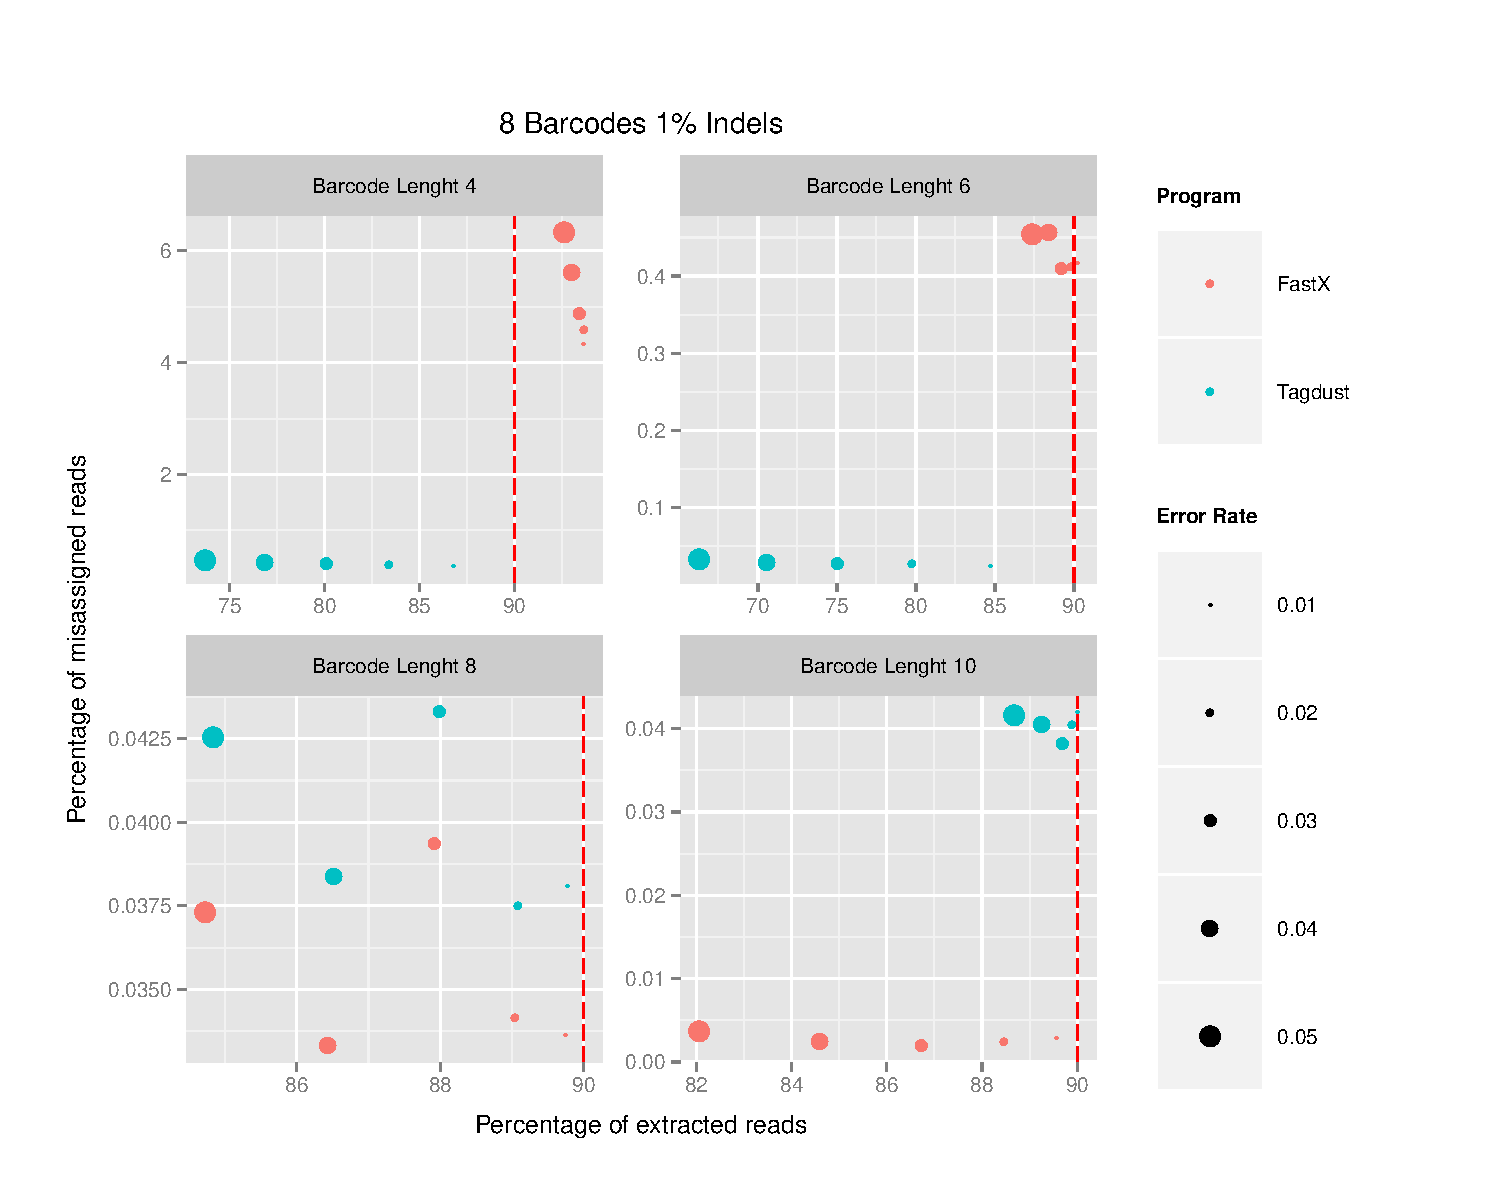
\includegraphics[scale = 0.35]{../figures/8Barcodes1Indels.pdf}
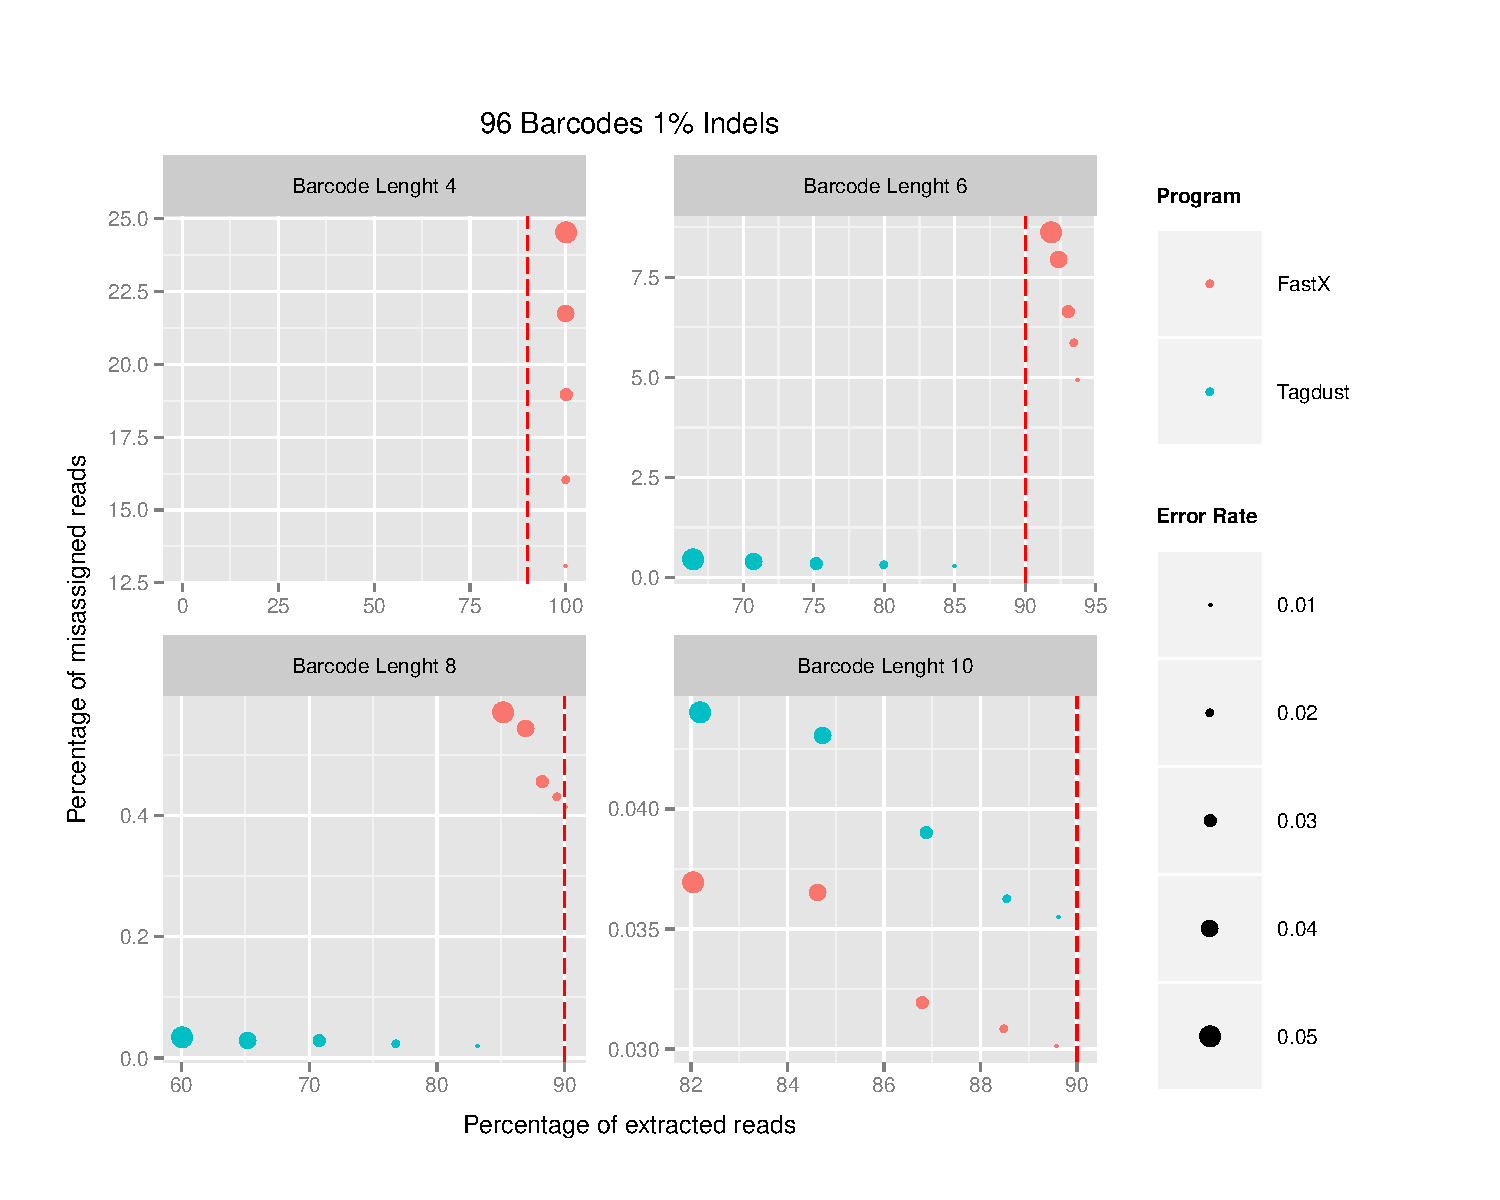
\includegraphics[scale = 0.35]{../figures/96Barcodes1Indels.pdf}
\end{center}
\caption{Performance of TagDust and Fastx at extracting reads containing 8 \textbf{(left)} and 96 \textbf{(right)} different barcodes. Different barcode lengths are shown in the different panels. The size of each datapoint represents the error rate ranging from 1 - 5\%.
}
\label{figure2}
\end{figure*}



\begin{table}[b]
\tableparts{%
\caption{This is a table caption}
\label{table:01}%
}{%
\begin{tabular*}{\columnwidth}{@{}lllll@{}}
\toprule
Col. head 1 & Col. head 2 & Col. head 3 & Col. head 4 & Col. head 5
\\
& (\%) & (s$^{-1}$) & (\%) & (s$^{-1}$)
\\
\colrule
Row 1 & Row 1 & Row 1 & -- & --
\\
Row 2 & Row 2 & Row 2 & Row 2 & Row 2
\\
\botrule
\end{tabular*}%
}
{This is a table footnote}
\end{table}


\subsection{Results subsection two}

Text.  Text. Text. Text. Text. Text. Text. Text. Text. Text. Text.
Text. Text. Text. Text. Text. Text. Text. Text. Text. Text. Text.
Text (see Table \ref{table:01}).

Text. Text. Text. Text. Text. Text.
Text. Text. Text. Text. Text. Text. Text. Text. Text. Text. Text.
Text. Text. Text. Text. Text. Text. Text. Text. Text.
Text (see Figure \ref{NAR-fig2}a).

Text. Text. Text. Text. Text.
Text. Text. Text. Text. Text. Text. Text. Text. Text. Text. Text.
Text. Text. Text. Text. Text. Text. Text. Text. Text. Text. Text.
Text. Text. Text. Text. Text. Text. Text. Text. Text. Text. Text.
Text. Text. Text. Text. Text. Text. Text. Text. Text. Text. Text.
Text. Text. Text. Text. Text. Text. Text. Text. Text. Text. Text.
Text. Text. Text. Text. Text. Text. Text. Text. Text. Text. Text.
Text. Text. Text. Text. Text. Text. Text. Text. Text. Text. Text.
Text. Text. Text. Text. Text. Text. Text. Text. Text. Text. Text.
Text. Text. Text. Text. Text. Text. Text. Text. Text. Text. Text.
Text. Text. Text. Text. Text. Text. Text. Text. Text. Text. Text.
Text. Text. Text. Text. Text. Text. Text. Text. Text. Text.

\begin{figure*}[t]
\begin{center}

\end{center}
\caption{Caption for wide figure over two columns.
\textbf{(a)} Left figure.
\textbf{(b)} Right figure (see (a)).
}
\label{NAR-fig2}
\end{figure*}


\subsection{Results subsection three}

Text. Text. Text. Text. Text. Text. Text. Text. Text. Text. Text.
Text. Text. Text. Text. Text. Text. Text. Text. Text. Text. Text.
Text. Text. Text. Text. Text. Text. Text. Text. Text. Text. Text.
Text. Text. Text. Text. Text. Text. Text. Text. Text. Text. Text.
Text. Text. Text. Text. Text. Text. Text. Text. Text. Text. Text.
Text. Text. Text. Text. Text. Text. Text. Text. Text. Text. Text.
Text. Text. Text. Text. Text. Text. Text. Text. Text. Text. Text.
Text. Text. Text. Text. Text. Text. Text. Text. Text. Text. Text.
Text. Text. Text. Text. Text. Text. Text. Text. Text. Text. Text.
Text. Text. Text. Text. Text. Text. Text. Text. Text. Text. Text.
Text. Text. Text.


\section{DISCUSSION}

\subsection{Discussion subsection one}

Text. Text. Text. Text. Text. Text. Text. Text. Text. Text. Text.
Text. Text. Text. Text. Text. Text. Text. Text. Text. Text. Text.
Text. Text. Text. Text. Text. Text. Text. Text. Text. Text. Text.
Text. Text. Text. Text. Text. Text. Text. Text. Text. Text. Text.
Text. Text. Text. Text. Text. Text. Text. Text. Text. Text. Text.
Text. Text. Text. Text. Text. Text. Text. Text. Text. Text. Text.
Text. Text. Text. Text. Text. Text. Text. Text. Text. Text. Text.
Text. Text. Text. Text. Text. Text. Text. Text. Text. Text. Text.
Text. Text. Text. Text. Text. Text. Text. Text. Text. Text. Text.
Text. Text. Text. Text. Text. Text. Text. Text. Text. Text. Text.
Text. Text. Text. Text. Text. Text. Text. Text. Text. Text. Text.
Text. Text. Text. Text. Text. Text. Text. Text. Text. Text. Text.
Text. Text. Text. Text. Text. Text. Text. Text. Text. Text. Text.
Text. Text. Text. Text. Text. Text. Text. Text. Text. Text. Text.
Text. Text. Text. Text. Text. Text. Text. Text. Text. Text. Text.
Text. Text. Text. Text. Text. Text. Text. Text. Text. Text. Text.
Text. Text. Text. Text. Text. Text. Text. Text. Text. Text. Text.
Text. Text. Text. Text. Text. Text. Text. Text. Text. Text. Text.
Text. Text. Text. Text. Text. Text. Text. Text. Text. Text. Text.
Text. Text. Text. Text. Text. Text. Text. Text. Text. Text. Text.
Text. Text. Text. Text. Text. Text.


\subsection{Discussion subsection two}

Text. Text. Text. Text. Text. Text. Text. Text. Text. Text. Text.
Text. Text. Text. Text. Text. Text. Text. Text. Text. Text. Text.
Text. Text. Text. Text. Text. Text. Text. Text. Text. Text. Text.
Text. Text. Text. Text. Text. Text. Text. Text. Text. Text. Text.
Text. Text. Text. Text. Text. Text. Text. Text. Text. Text. Text.
Text. Text. Text. Text. Text. Text. Text. Text. Text. Text. Text.
Text. Text. Text. Text. Text. Text. Text. Text. Text. Text. Text.
Text. Text. Text. Text. Text. Text. Text. Text. Text. Text. Text.
Text. Text. Text. Text. Text. Text. Text. Text. Text. Text. Text.
Text. Text. Text. Text. Text. Text. Text. Text. Text. Text. Text.
Text.

Text. Text. Text. Text. Text. Text. Text. Text. Text. Text. Text.
Text. Text. Text. Text. Text. Text. Text. Text. Text. Text. Text.
Text. Text. Text. Text. Text. Text. Text. Text. Text. Text. Text.
Text. Text. Text. Text. Text. Text. Text. Text. Text. Text. Text.
Text. Text. Text. Text. Text. Text. Text. Text. Text. Text. Text.
Text. Text. Text. Text. Text. Text. Text. Text. Text. Text. Text.
Text. Text. Text. Text. Text. Text. Text. Text. Text. Text. Text.
Text. Text. Text. Text. Text. Text. Text. Text. Text. Text. Text.
Text. Text. Text. Text. Text. Text. Text. Text. Text. Text. Text.
Text. Text. Text. Text. Text. Text. Text. Text. Text. Text. Text.
Text. Text. Text. Text. Text. Text. Text. Text. Text. Text.


\begin{figure}[t]
\begin{center}
\includegraphics{NAR-fig1.eps}
\end{center}
\caption{Caption for figure within column.}
\label{NAR-fig1}
\end{figure}

\subsection{Discussion subsection three}

Text. Text. Text. Text. Text. Text. Text. Text. Text. Text. Text.
Text. Text. Text. Text. Text. Text. Text. Text. Text. Text. Text.
Text. Text. Text. Text. Text. Text. Text. Text. Text. Text. Text.
Text. Text. Text. Text. Text. Text. Text. Text. Text. Text. Text.
Text. Text. Text. Text. Text. Text. Text. Text. Text. Text. Text.
Text. Text. Text. Text. Text. Text. Text. Text. Text. Text. Text.
Text. Text. Text. Text. Text. Text. Text. Text. Text. Text. Text.
Text. Text. Text. Text. Text. Text. Text. Text. Text. Text. Text.
Text. Text. Text. Text. Text. Text. Text. Text. Text. Text. Text.
Text. Text. Text. Text. Text. Text. Text. Text. Text. Text. Text.
Text. Text. Text. Text. Text. Text. Text. Text. Text.

Text. Text. Text. Text. Text. Text. Text. Text. Text. Text. Text.
Text. Text. Text. Text. Text. Text. Text. Text. Text. Text. Text.
Text. Text. Text. Text. Text. Text. Text. Text. Text. Text. Text.
Text. Text. Text. Text. Text. Text. Text. Text. Text. Text. Text.
Text. Text. Text. Text. Text. Text. Text. Text. Text. Text. Text.
Text. Text. Text. Text. Text. Text. Text. Text. Text. Text. Text.
Text. Text. Text. Text. Text. Text. Text. Text. Text. Text. Text.
Text. Text. Text. Text. Text. Text. Text.

Text. Text. Text. Text. Text. Text. Text. Text. Text. Text. Text.
Text. Text. Text. Text. Text. Text. Text. Text. Text. Text. Text.
Text. Text. Text. Text. Text. Text. Text. Text. Text. Text. Text.
Text. Text. Text. Text. Text. Text. Text. Text. Text. Text. Text.
Text. Text. Text. Text. Text. Text. Text. Text. Text. Text. Text.
Text. Text. Text. Text. Text. Text. Text. Text. Text. Text. Text.
Text. Text. Text. Text. Text. Text. Text. Text. Text. Text. Text.
Text. Text. Text. Text. Text. Text. Text.


\section{CONCLUSION}

Text. Text. Text. Text. Text. Text. Text. Text. Text. Text. Text.
Text. Text. Text. Text. Text. Text. Text. Text. Text. Text. Text.
Text. Text. Text. Text. Text. Text. Text. Text. Text. Text. Text.
Text. Text. Text. Text. Text. Text. Text. Text. Text. Text. Text.
Text. Text. Text. Text. Text. Text. Text. Text. Text. Text. Text.
Text. Text. Text. Text. Text. Text. Text. Text. Text. Text. Text.
Text. Text. Text. Text. Text. Text. Text. Text. Text. Text. Text.
Text. Text. Text. Text. Text. Text. Text. Text. Text. Text. Text.
Text. Text. Text. Text. Text. Text. Text. Text. Text. Text. Text.
Text. Text. Text.


\section{ACKNOWLEDGEMENTS}

Text. Text. Text. Text. Text. Text. Text. Text. Text. Text. Text.
Text. Text. Text. Text.


\subsubsection{Conflict of interest statement.} None declared.
\newpage


\begin{thebibliography}{4}

% Format for article
\bibitem{1}
Author,A.B. and Author,C. (1992)
Article title.
\textit{Abbreviated Journal Name}, \textbf{5}, 300--330.

% Format for book
\bibitem{2}
Author,D., Author,E.F. and Author,G. (1995)
\textit{Book Title}.
Publisher Name, Publisher Address.

% Format for chapter in book
\bibitem{3}
Author,H. and Author,I. (2005)
Chapter title.
In
Editor,A. and Editor,B. (eds),
\textit{Book Title},
Publisher Name, Publisher Address,
pp.\ 60--80.

% Another article
\bibitem{4}
Author,Y. and Author,Z. (2002)
Article title.
\textit{Abbreviated Journal Name}, \textbf{53}, 500--520.




%@article{Kivioja:2012kg,
%author = {Kivioja, Teemu and V{\"a}h{\"a}rautio, Anna and Karlsson, Kasper and Bonke, Martin and Enge, %Martin and Linnarsson, Sten and Taipale, Jussi},
%title = {{Counting absolute numbers of molecules using unique molecular identifiers.}},
%journal = {Nature methods},
%year = {2012},
%volume = {9},
%number = {1},
%pages = {72--74},
%month = jan
%}


%@book{durbin,
%    author = {Durbin, R. and Eddy, S. and Krogh, A. and Mitchison, G.},
%    edition = {eleventh},
%publisher = {Press, Cambridge U.},
%    title = {{Biological sequence analysis}},
%    year = {2006}
%}



%@article{Kall:2005vg,
%author = {K{\"a}ll, Lukas and Krogh, Anders and Sonnhammer, Erik L L},
%title = {{An HMM posterior decoder for sequence feature prediction that includes homology information}},
%journal = {Bioinformatics (Oxford, England)},
%year = {2005}
%}




\end{thebibliography}

\end{document}
